\documentclass[11pt]{article}

\usepackage[letterpaper,bindingoffset=0.2in,
            left=1in,right=1in,top=1in,bottom=1in,
            footskip=.25in]{geometry}

\usepackage{hyperref}
	\hypersetup{
			colorlinks=true,
			linkcolor=black,
			filecolor=magenta,      
			urlcolor=blue,
	}
	
\usepackage{graphicx}
	\graphicspath{ {images/} }
	
\usepackage{subcaption}

\usepackage{float}
	
\begin{document}


\title{COMP SCI 5401 FS2017 Assignment 1d}
\author{Stuart Miller\\\href{mailto:sm67c@mst.edu}{sm67c@mst.edu}}
\maketitle


\section{Overview}\label{sect:overview}

For assignment 1d, this iteration of the Stock-Cutting evolutionary algorithm introduces two new fitness measures: width and edge length. The main focus will be on length and width, while edge length will be discussed in Section \ref{sect:bonus3} (Bonus 3).
In order to facilitate this, a structure was created to hold various fitness measures and configuration options were added to point objective accessory to the configured fitness. The bulk of this assignment uses length as objective 1 and width as objective 2. For all of the fitness measures, minimized values were recorded by subtracting the observed measure from a set maximum value.

\section{Configuration 1}\label{sect:cfg1}

For the first configuration, a highly selective EA will be employed. This EA uses k-tournaments with selection from a greedy 100\% of the population. This is likely to allow the EA to get locked into a particular solution and not allow for innovation into possibly more optimal areas of the fitness landscape. A control group was also evaluated, where each EA had a k-tournament with selection from 50\% of the population.

Figure \ref{fig:cfg1_best} shows the best fitness for each objective. (Again, objective 1 is set to length and objective 2 is set to width.) The control group shows that it is able to usually generate better solutions, although not always. The greedy version of set 1 averaged a better best width, and the greedy versions of set 3 managed to find a single solution that was had a slightly better length than the control. In general though, it is clear that the greedy k-tournaments perform worse.

Figure \ref{fig:cfg1_pareto} shows the points on the Pareto front. Note that the Pareto front is quite sparse. This is likely due to the specified way in which best Pareto fronts are determined. If a higher percentage of states in one Pareto front dominate the other than vice-versa, it is considered better. This gives an advantage to small Pareto fronts. For example a front with 3 solutions, 2 of which dominate is considered better than a front with 10 solutions, 6 of which dominate. Even though the 10 solution front has many more solutions, 3 solution front has a higher ratio and thus, wins.

\begin{figure}[H]
	\centering
  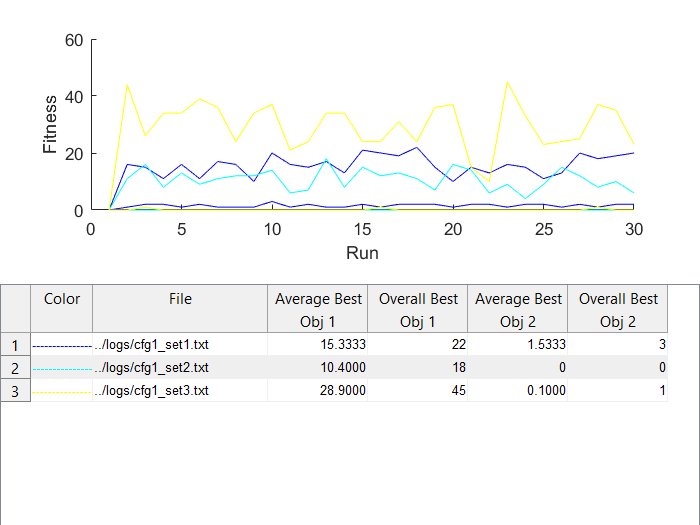
\includegraphics[width=5in]{assn1d_cfg1_bestfitness.png}
  \captionof{figure}{Configuration 1 Best Per-Objective Fitness}
  \label{fig:cfg1_best}
\end{figure}

\begin{figure}[H]
	\centering
  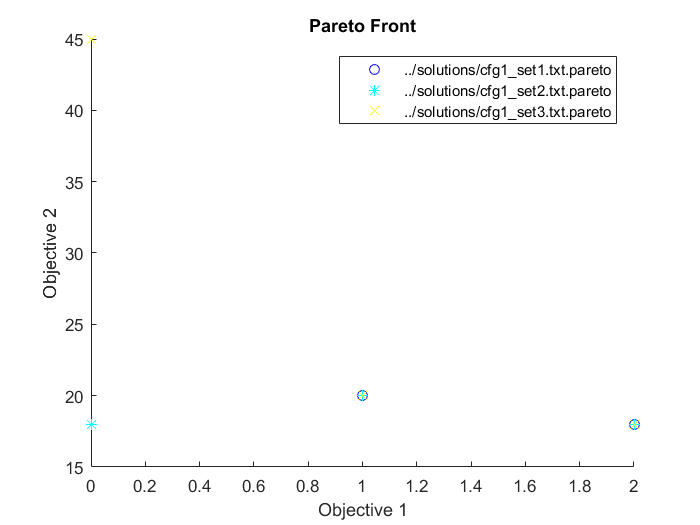
\includegraphics[width=4in]{assn1d_cfg1_pareto.png}
  \captionof{figure}{Configuration 1 Pareto Fronts}
  \label{fig:cfg1_pareto}
\end{figure}

\section{Configuration 2}\label{sect:cfg2}

The second configuration examines the effect of mutation rate. Three groups were used: one with no mutation at all, one with a 50\% mutation chance, and one where every state was mutated once. Creep mutations were used, so each shape has a chance to change a single parameter up to 2 units in any direction. All other parameters were kept the same.

It is interesting that the fitness graph in Figure \ref{fig:cfg2_best} show almost no difference in best fitness. The 50\% mutation rate returns slightly better fitnesses, but not by much. This could be due to the fact the repair function takes care of creep on its own by moving the shapes a small amount. Adding a creep mutation seems to have little additional benefit. The benefit that is seen is likely due to the 50\% mutation allowing for slightly increased exploration of the fitness landscape, while the 100\% mutation provides to little direction to settle on definitively better solutions. Again, it is hard to see improvements in width due to the complexity of the data sets. Furthemore, smaller improvements are seen by the more complex data sets due to their increased complexity.

Due to the lack of diversity in widths, the Pareto fronts shown in Figure \ref{fig:cfg2_pareto} tend to be small, showing points at the 0, 1, and 2 width measures.

\begin{figure}[H]
	\centering
  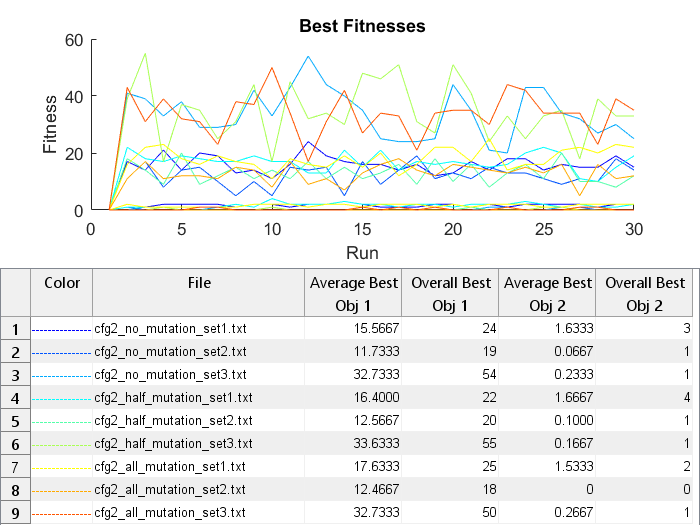
\includegraphics[width=5in]{assn1d_cfg2_bestfitness.png}
  \captionof{figure}{Configuration 2 Best Per-Objective Fitness}
  \label{fig:cfg2_best}
\end{figure}

\begin{figure}[H]
	\centering
  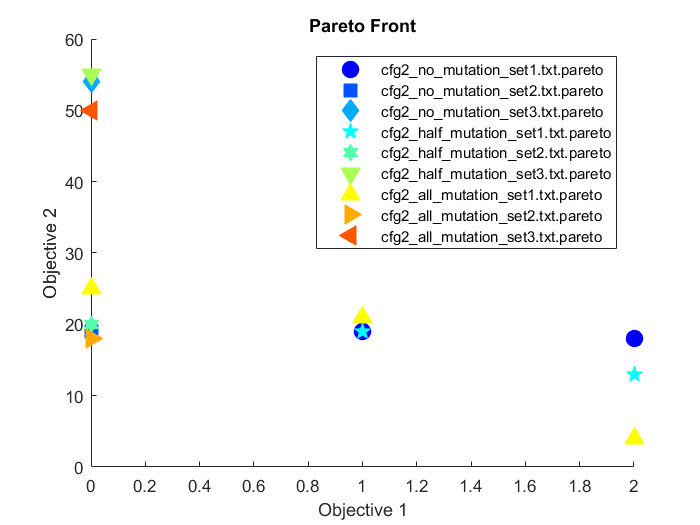
\includegraphics[width=4in]{assn1d_cfg2_pareto.png}
  \captionof{figure}{Configuration 2 Pareto Fronts}
  \label{fig:cfg2_pareto}
\end{figure}

\section{Configuration 3}\label{sect:cfg3}

Finally, the third configuration toggles the repair function. Calling the repair function was compared to using random resets for invalid shape placements.

This configuration displays undoubtedly the largest divide yet. Figure \ref{fig:cfg3_best} shows a clear difference between the fitnesses from repair constraint resolution verses the random reset constraint resolution. This divide is a little less clear in the second objective (width), although this is in line with the difficulty to establish any significant improvements in width across the other configurations run above. As is to be expected, the more complex data sets show lesser improvements with set 2 having a very low improvement.

Again, the Pareto fronts shown in Figure \ref{fig:cfg3_pareto} have few members, showing peaks at the 0 and 1 widths and a few at 2.

\begin{figure}[H]
	\centering
  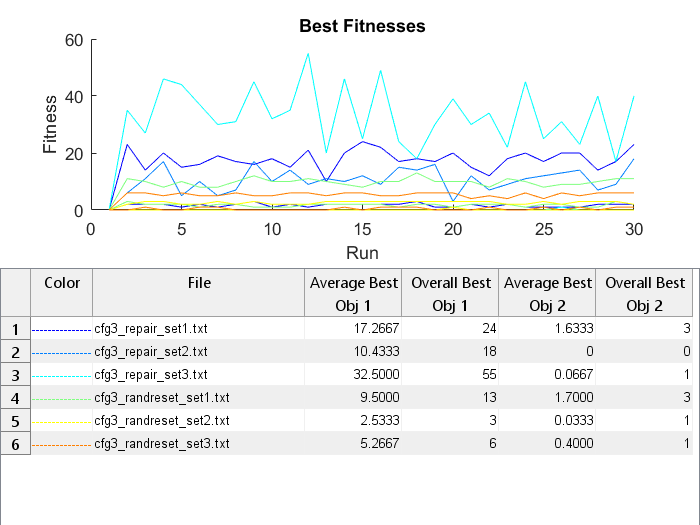
\includegraphics[width=5in]{assn1d_cfg3_bestfitness.png}
  \captionof{figure}{Configuration 3 Best Per-Objective Fitness}
  \label{fig:cfg3_best}
\end{figure}

\begin{figure}[H]
	\centering
  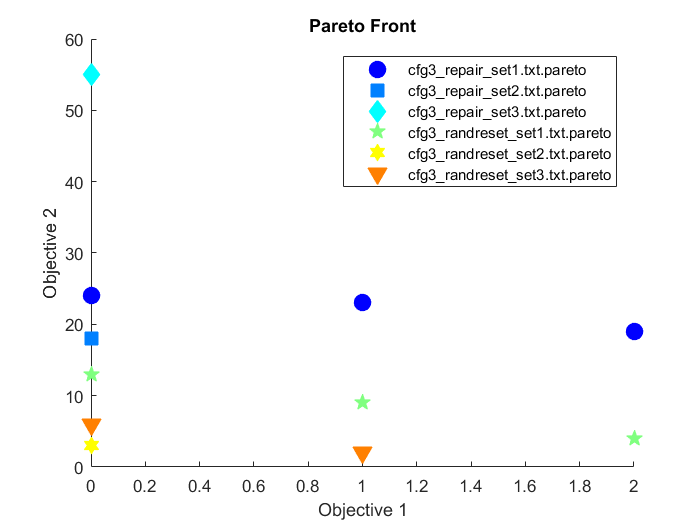
\includegraphics[width=4in]{assn1d_cfg3_pareto.png}
  \captionof{figure}{Configuration 3 Pareto Fronts}
  \label{fig:cfg3_pareto}
\end{figure}

\section{Bonus 3}\label{sect:bonus3}

Bonus 3 adds in another objective: edges (or glass-cut). Objective 1 was set to length as before and objective 2 was changed to edge length. This was achieved by counting the perimeter of each shape while discounting those edges that were shared with either the edge of the stock or another shape. In order to provide an objective to minimize, the first call to the edge calculating function stores its calculated value and subtracts all subsequent values from that. This works because our first generation is theoretically the most unfit with improvements occurring from there.

The best fitnesses plot in Figure \ref{fig:bonus3_best} shows that the edge lengths were quite diverse across all test sets. This makes sense as the more complex sets are going to have longer edge lengths to start with. Unfortunately, this makes it quite difficult to observe any changes in length (objective 1). The table makes it clear that some improvements are still made, but the best lengths are considerably less than the control runs from earlier (see Figure \ref{fig:cfg1_best}). 

The Pareto front plot in Figure \ref{fig:bonus3_pareto} is much more enlightening though. Whereas before, the choice of width as a second objective limited fronts to only a few values (as widths were never able to improve beyond 2), edge lengths are now much more varied, allowing for expanded Pareto fronts. Here, it is easy to see the diagonals that form the front for each data set.

\begin{figure}[H]
	\centering
  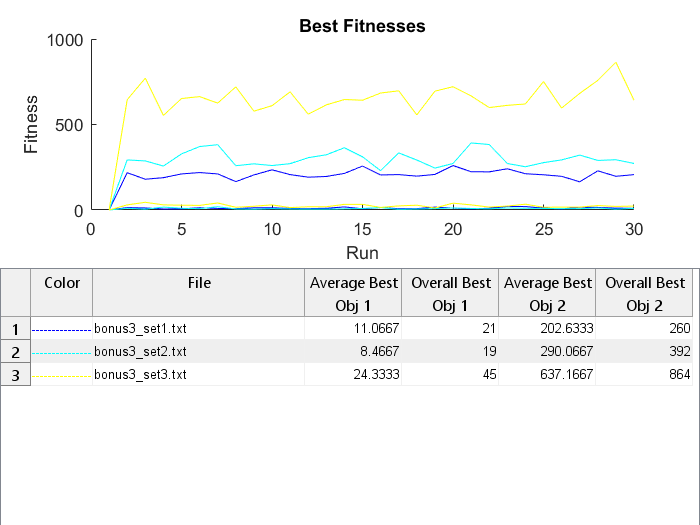
\includegraphics[width=5in]{assn1d_bonus3_bestfitness.png}
  \captionof{figure}{Bonus 3 Best Per-Objective Fitness}
  \label{fig:bonus3_best}
\end{figure}

\begin{figure}[H]
	\centering
  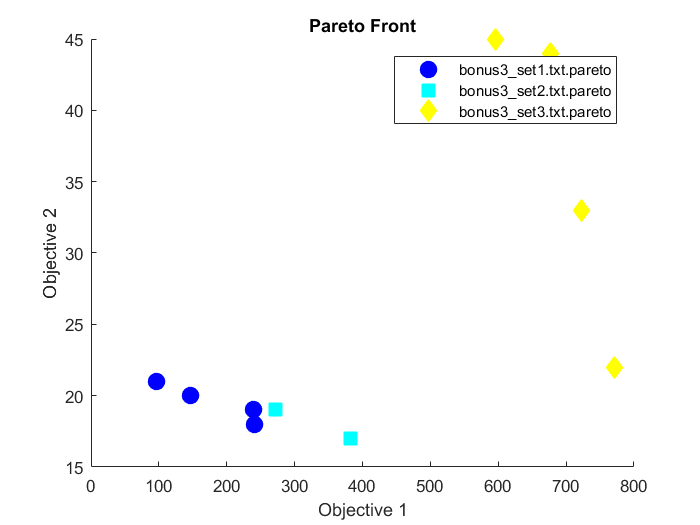
\includegraphics[width=4in]{assn1d_bonus3_pareto.png}
  \captionof{figure}{Bonus 3 Pareto Fronts}
  \label{fig:bonus3_pareto}
\end{figure}

\end{document}